\newpage
\subsection{QuizziPedia::Front-End::Controllers}


\begin{figure}
	\centering
	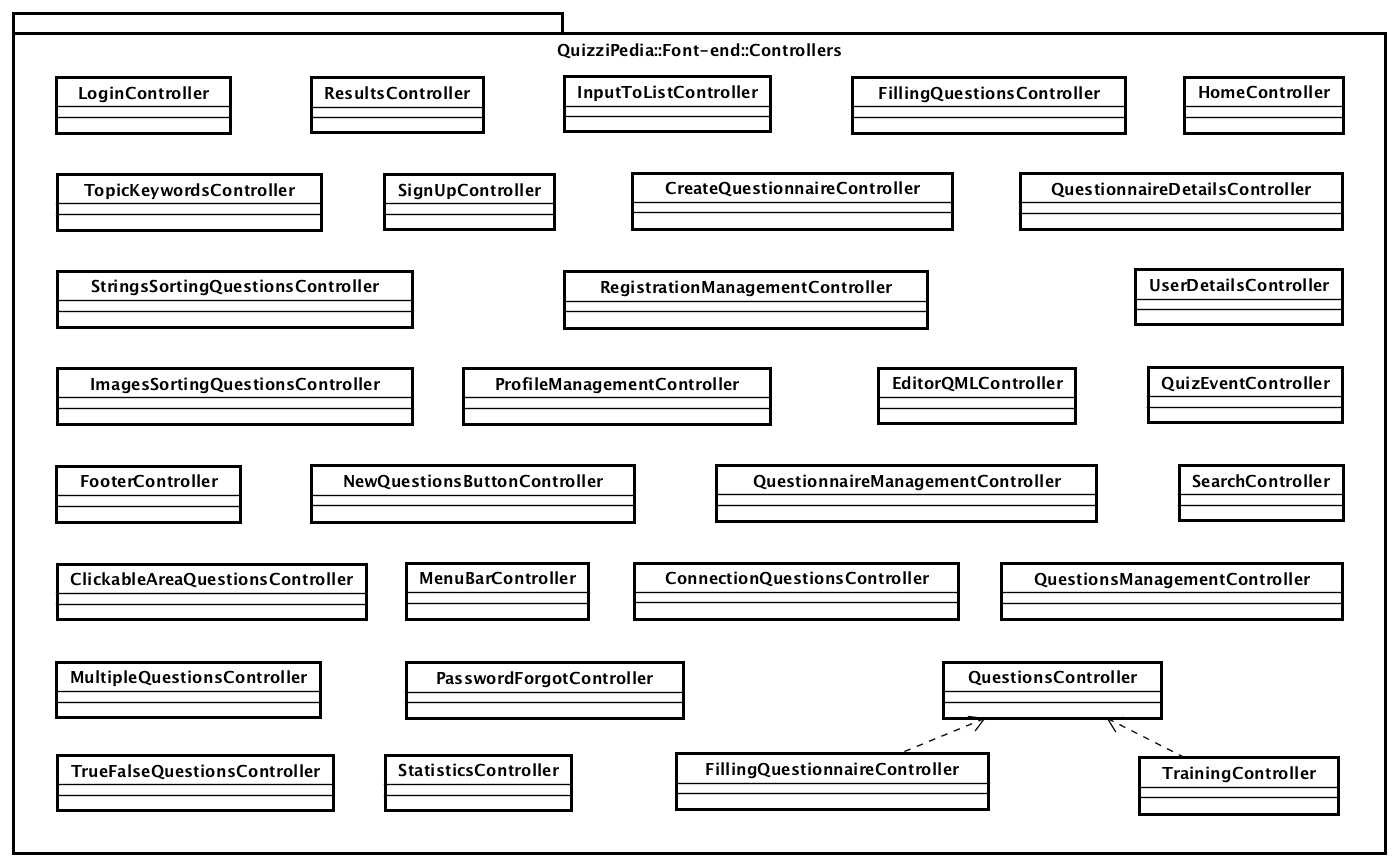
\includegraphics[scale=0.45]{UML/Package/QuizziPedia_Front-End_Controllers.png}
	\caption{QuizziPedia::Front-End::Controllers::SignUpController}
\end{figure}

\subsubsection{Informazioni generali}
\begin{itemize}
	\item \textbf{Descrizione}: package che contiene i controller individuati per la parte front-end dell'applicazione;
	\item \textbf{Padre:} \texttt{Front-End};
	\item \textbf{Interazione con altri componenti:}
	\begin{itemize}
		\item \texttt{Models} - package che contiene le classi model individuate;
		\item \texttt{Services} - package che contiene le classi services individuate.
	\end{itemize} 
\end{itemize}
\subsubsection{Classi}

\paragraph{QuizziPedia::Front-End::Controllers::LoginController}
\begin{figure}
	\centering
	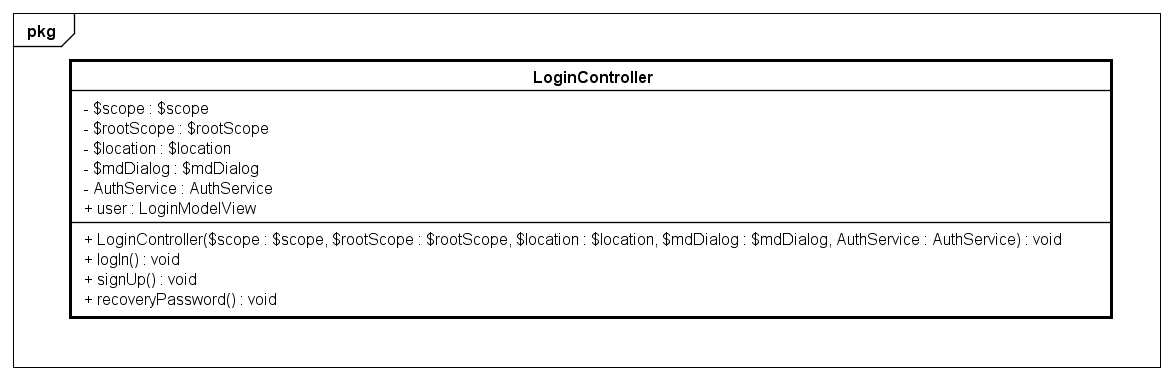
\includegraphics[scale=0.45]{UML/Classi/Front-End/QuizziPedia_Front-end_Controller_LoginController.png}
	\caption{QuizziPedia::Front-End::Controllers::LoginController}
\end{figure}
\begin{itemize}
	\item \textbf{Descrizione}: questa classe permette di gestire l'autenticazione dell'utente al sistema; 
	\item \textbf{Utilizzo}: fornisce le funzionalità di autenticazione al sistema, compresa la gestione di situazioni di errore autenticazione;
	\item \textbf{Relazione con altre classi:}
	\begin{itemize}
		\item \textit{IN} \texttt{LoginView}: view contenente le form necessarie per effettuare il login. Contiene inoltre un link alla pagina di registrazione e uno alla pagina per il recupero della password;
		\item \textit{OUT} \texttt{LangService}: questa classe permette di gestire la lingua nella quale si è scelto di utilizzare l'applicazione;
		\item \textit{OUT} \texttt{AuthService}: questa classe permette di gestire la registrazione e l'autenticazione di un utente;
		\item \textit{OUT} \texttt{ErrorController}: questa classe permette di gestire tutti i messaggi di errore da mostrare all'utente.

	\end{itemize}
	\item \textbf{Attributi:}
	\begin{itemize}
		\item 
	\end{itemize}
	\item \textbf{Metodi:}
	\begin{itemize}
		\item 
	\end{itemize}
\end{itemize}

\paragraph{QuizziPedia::Front-End::Controllers::SignUpController}
\begin{figure}
	\centering
	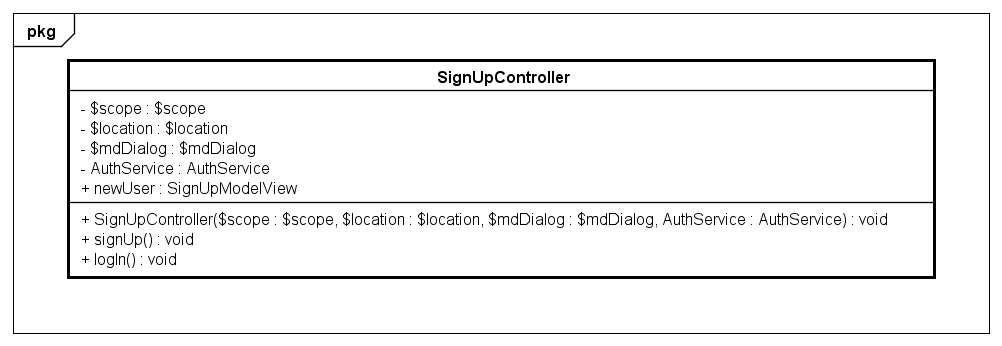
\includegraphics[scale=0.45]{UML/Classi/Front-End/QuizziPedia_Front-end_Controller_SignUpController.png}
	\caption{QuizziPedia::Front-End::Controllers::SignUpController}
\end{figure}
\begin{itemize}
	\item \textbf{Descrizione}: questa classe permette di gestire la registrazione di un utente al sistema;
	\item \textbf{Utilizzo}: fornisce le funzionalità di registrazione di un utente al sistema;
	\item \textbf{Relazione con altre classi:}
	\begin{itemize}
		\item \textit{IN} \texttt{SignUpView}: view contenente le form dedicate alla registrazione utente. Contiene inoltre un link alla pagina di login;
		\item \textit{OUT} \texttt{AuthService}: questa classe permette di gestire la registrazione e l'autenticazione di un utente;
		\item \textit{OUT} \texttt{LangService}: questa classe permette di gestire la lingua nella quale si è scelto di utilizzare l'applicazione;
		\item \textit{OUT} \texttt{ErrorController}: questa classe permette di gestire tutti i messaggi di errore da mostrare all'utente.
	\end{itemize}
	\item \textbf{Attributi:}
	\begin{itemize}
		\item 
	\end{itemize}
	\item \textbf{Metodi:}
	\begin{itemize}
		\item 
	\end{itemize}
\end{itemize}

\paragraph{QuizziPedia::Front-End::Controllers::HomeController}
\begin{figure}
	\centering
	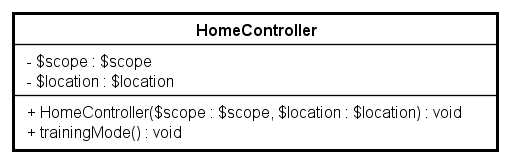
\includegraphics[scale=0.45]{UML/Classi/Front-End/QuizziPedia_Front-end_Controller_HomeController.png}
	\caption{QuizziPedia::Front-End::Controllers::HomeController}
\end{figure}
\begin{itemize}
	\item \textbf{Descrizione}: questa classe permette di gestire la home page;
	\item \textbf{Utilizzo}: fornisce tutte le informazioni da mostrare nella homepage;
	\item \textbf{Relazione con altre classi:}
	\begin{itemize}
		\item \textit{IN} \texttt{HomeView}: view contenente la barra di ricerca per gli utenti e questionari e il bottone che porterà l'utente nella modalità allenamento;
		\item \textit{OUT} \texttt{LangService}: questa classe permette di gestire la lingua nella quale si è scelto di utilizzare l'applicazione;
		\item \textit{OUT} \texttt{ErrorController}: questa classe permette di gestire tutti i messaggi di errore da mostrare all'utente.
	\end{itemize}
	\item \textbf{Attributi:}
	\begin{itemize}
		\item 
	\end{itemize}
	\item \textbf{Metodi:}
	\begin{itemize}
		\item 
	\end{itemize}
\end{itemize}

\paragraph{QuizziPedia::Front-End::Controllers::SearchController}
\begin{figure}
	\centering
	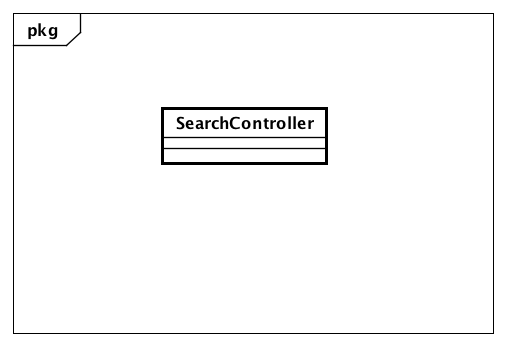
\includegraphics[scale=0.45]{UML/Classi/Front-End/QuizziPedia_Front-end_Controller_SearchController.png}
	\caption{QuizziPedia::Front-End::Controllers::SearchController}
\end{figure}
\begin{itemize}
	\item \textbf{Descrizione}: questa classe permette di gestire la ricerca di questionari e utenti all'interno dell'applicazione;
	\item \textbf{Utilizzo}: fornisce all'utente le funzionalità di ricerca per utenti e questionari;
	\item \textbf{Relazione con altre classi:}
	\begin{itemize}
		\item \textit{OUT} \texttt{ResultsView}: view contenente i risultati della ricerca effettuata, sia gli utenti che i questionari;
		\item \textit{OUT} \texttt{ErrorController}: questa classe permette di gestire tutti i messaggi di errore da mostrare all'utente;
		\item \textit{OUT} \texttt{UserDetailsService}: questa classe permette di ottenere i dati personali degli utenti;
		\item \textit{OUT} \texttt{QuizService}: questa classe permette di ottenere i dati di un quiz tramite delle parole chiave inserite dall'utente nella barra di ricerca;
		\item \textit{OUT} \texttt{LangService}: questa classe permette di gestire la lingua nella quale si è scelto di utilizzare l'applicazione.
	\end{itemize}
	\item \textbf{Attributi:}
	\begin{itemize}
		\item 
	\end{itemize}
	\item \textbf{Metodi:}
	\begin{itemize}
		\item 
	\end{itemize}
\end{itemize}

\paragraph{QuizziPedia::Front-End::Controllers::ProfileManagementController}
\begin{figure}
	\centering
	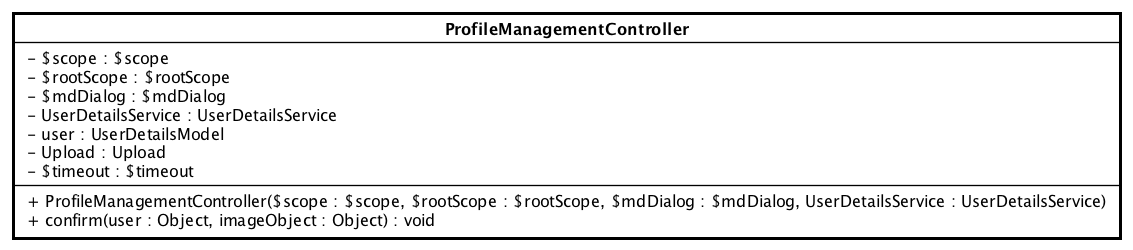
\includegraphics[scale=0.45]{UML/Classi/Front-End/QuizziPedia_Front-end_Controller_ProfileManagementController.png}
	\caption{QuizziPedia::Front-End::Controllers::ProfileManagementController}
\end{figure}
\begin{itemize}
	\item \textbf{Descrizione}: questa classe permette di gestire il profilo personale di un utente; 
	\item \textbf{Utilizzo}: fornisce le funzionalità all'utente per poter gestire i propri dati;
	\item \textbf{Relazione con altre classi:}
	\begin{itemize}
		\item \textit{IN} \texttt{ProfileManagementView}: view contenente i dati personali che un utente può modificare dopo essersi registrato al sistema;
		\item \textit{OUT} \texttt{UserDetailsService}: questa classe permette di ottenere i dati personali degli utenti;
		\item \textit{OUT} \texttt{LangService}: questa classe permette di gestire la lingua nella quale si è scelto di utilizzare l'applicazione;
		\item \textit{OUT} \texttt{ErrorController}: questa classe permette di gestire tutti i messaggi di errore da mostrare all'utente.
	\end{itemize}
	\item \textbf{Attributi:}
	\begin{itemize}
		\item 
	\end{itemize}
	\item \textbf{Metodi:}
	\begin{itemize}
		\item 
	\end{itemize}
\end{itemize}

\paragraph{QuizziPedia::Front-End::Controllers::LogoutController}
\begin{figure}
	\centering
	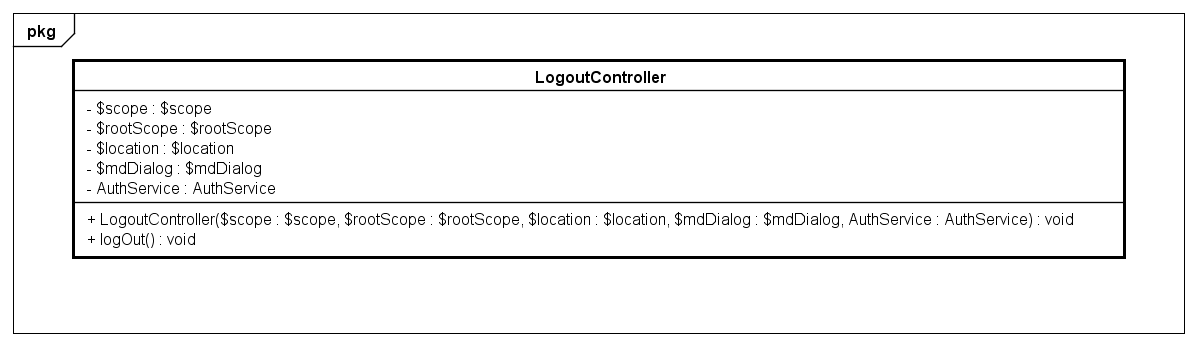
\includegraphics[scale=0.45]{UML/Classi/Front-End/QuizziPedia_Front-end_Controller_LogoutController.png}
	\caption{QuizziPedia::Front-End::Controllers::LogoutController}
\end{figure}
\begin{itemize}
	\item \textbf{Descrizione}: questa classe permette di gestire la pagina di logout;
	\item \textbf{Utilizzo}: fornisce la funzionalità per effettuare il logout dall'applicazione;
	\item \textbf{Relazione con altre classi:}
	\begin{itemize}
		\item \textit{OUT} \texttt{MenuBarDirective}: rappresenta il menù, presente in ogni pagina dell'applicazione, generato in base agli oggetti passati nello \$scope isolato. Fornisce un pulsante per ogni oggetto ricevuto come parametro, ogni pulsante viene rappresentato con un’icona e con un testo. Al click di un pulsante viene invocata la funzione ad esso associata;
		\item \textit{OUT} \texttt{AuthService}: questa classe permette di gestire la registrazione e l'autenticazione di un utente;
		\item \textit{OUT} \texttt{LangService}: questa classe permette di gestire la lingua nella quale si è scelto di utilizzare l'applicazione;
		\item \textit{OUT} \texttt{ErrorController}: questa classe permette di gestire tutti i messaggi di errore da mostrare all'utente.
	\end{itemize}
	\item \textbf{Attributi:}
	\begin{itemize}
		\item 
	\end{itemize}
	\item \textbf{Metodi:}
	\begin{itemize}
		\item 
	\end{itemize}
\end{itemize}

\paragraph{QuizziPedia::Front-End::Controllers::PasswordForgotController}
\begin{figure}
	\centering
	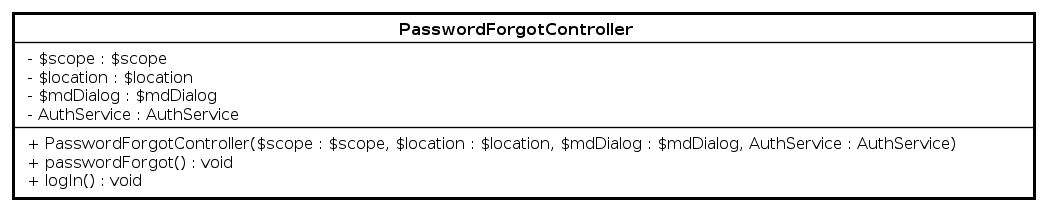
\includegraphics[scale=0.45]{UML/Classi/Front-End/QuizziPedia_Front-end_Controller_PasswordForgotController.png}
	\caption{QuizziPedia::Front-End::Controllers::PasswordForgotController}
\end{figure}
\begin{itemize}
	\item \textbf{Descrizione}: questa classe permette di gestire il ripristino della password dimenticata;
	\item \textbf{Utilizzo}: fornisce tutte le funzionalità per ripristinare la password dopo aver verificato l'identità dell'utente;
	\item \textbf{Relazione con altre classi:}
	\begin{itemize}
		\item \textit{IN} \texttt{PasswordForgotView}: view contenente le form necessarie per il recupero della password dimenticata; 
		\item \textit{OUT} \texttt{AuthService}: questa classe permette di gestire la registrazione e l'autenticazione di un utente;
		\item \textit{OUT} \texttt{LangService}: questa classe permette di gestire la lingua nella quale si è scelto di utilizzare l'applicazione;
		\item \textit{OUT} \texttt{ErrorController}: questa classe permette di gestire tutti i messaggi di errore da mostrare all'utente.
	\end{itemize}
	\item \textbf{Attributi:}
	\begin{itemize}
		\item 
	\end{itemize}
	\item \textbf{Metodi:}
	\begin{itemize}
		\item 
	\end{itemize}
\end{itemize}

\paragraph{QuizziPedia::Front-End::Controllers::TrueFalseQuestionsController}
\begin{figure}
	\centering
	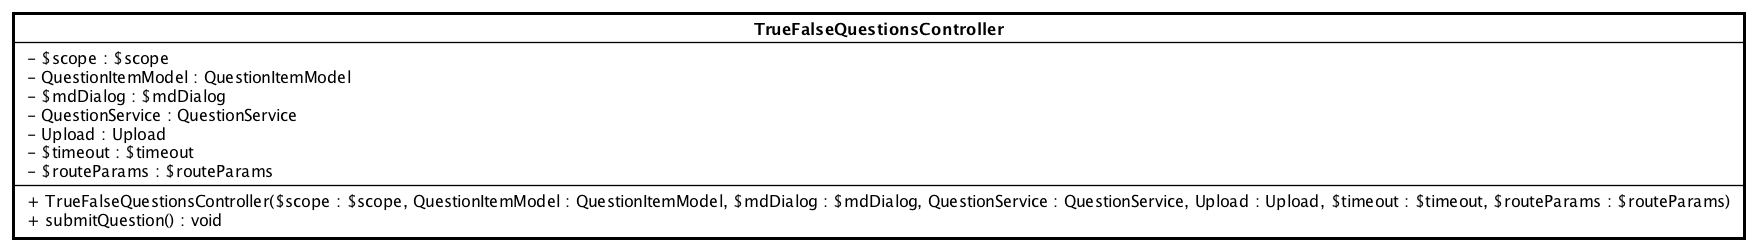
\includegraphics[scale=0.45]{UML/Classi/Front-End/QuizziPedia_Front-end_Controller_TrueFalseQuestionsController.png}
	\caption{QuizziPedia::Front-End::Controllers::TrueFalseQuestionsController}
\end{figure}
\begin{itemize}
	\item \textbf{Descrizione}: questa classe permette di gestire la creazione e la modifica di una domanda vero/falso;
	\item \textbf{Utilizzo}: fornisce le funzionalità per inserire una nuova domanda vero/falso nel database e per modificarne una esistente;
	\item \textbf{Relazione con altre classi:}
	\begin{itemize}
		\item \textit{IN} \texttt{TrueFalseQuestionsView}: view contenente i campi per creare una domanda vero/falso;  
		\item \textit{OUT} \texttt{LangService}: questa classe permette di gestire la lingua nella quale si è scelto di utilizzare l'applicazione;
		\item \textit{OUT} \texttt{QuestionService}: questa classe permette di ottenere domande esistenti e salvare nuove domande;
		\item \textit{OUT} \texttt{ErrorController}: questa classe permette di gestire tutti i messaggi di errore da mostrare all'utente.
	\end{itemize}
	\item \textbf{Attributi:}
	\begin{itemize}
		\item 
	\end{itemize}
	\item \textbf{Metodi:}
	\begin{itemize}
		\item 
	\end{itemize}
\end{itemize}

\paragraph{QuizziPedia::Front-End::Controllers::MultipleQuestionsController}
\begin{figure}
	\centering
	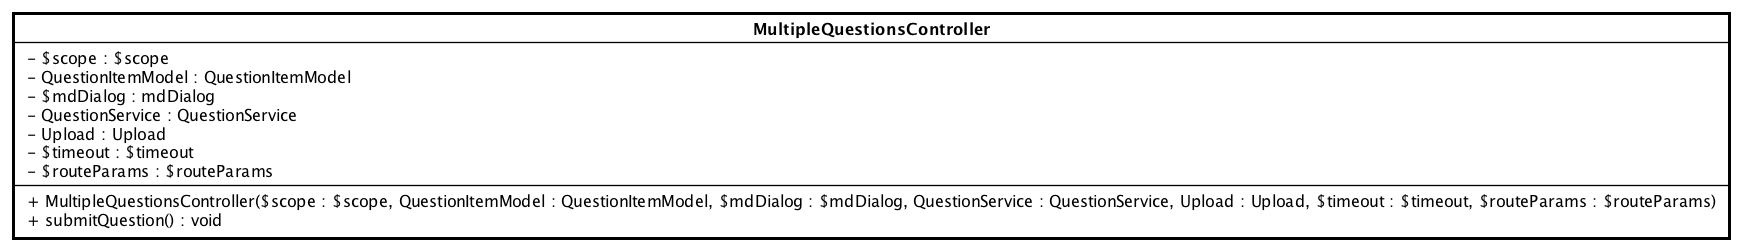
\includegraphics[scale=0.45]{UML/Classi/Front-End/QuizziPedia_Front-end_Controller_MultipleQuestionsController.png}
	\caption{QuizziPedia::Front-End::Controllers::MultipleChoiceQuestion}
\end{figure}
\begin{itemize}
	\item \textbf{Descrizione}: questa classe permette di gestire la creazione e la modifica di una domanda a risposta multipla;
	\item \textbf{Utilizzo}: fornisce le funzionalità per inserire una nuova domanda a risposta multipla nel database e per modificarne una esistente;
	\item \textbf{Relazione con altre classi:}
	\begin{itemize}
		\item \textit{IN} \texttt{MultipleQuestionsView}: view contenente i campi per creare una domanda a risposta multipla;  
		\item \textit{OUT} \texttt{LangService}: questa classe permette di gestire la lingua nella quale si è scelto di utilizzare l'applicazione;
		\item \textit{OUT} \texttt{QuestionService}: questa classe permette di ottenere domande esistenti e salvare nuove domande;
		\item \textit{OUT} \texttt{ErrorController}: questa classe permette di gestire tutti i messaggi di errore da mostrare all'utente.
	\end{itemize}
	\item \textbf{Attributi:}
	\begin{itemize}
		\item 
	\end{itemize}
	\item \textbf{Metodi:}
	\begin{itemize}
		\item 
	\end{itemize}
\end{itemize}

\paragraph{QuizziPedia::Front-End::Controllers::ConnectionQuestionsController}
\begin{figure}
	\centering
	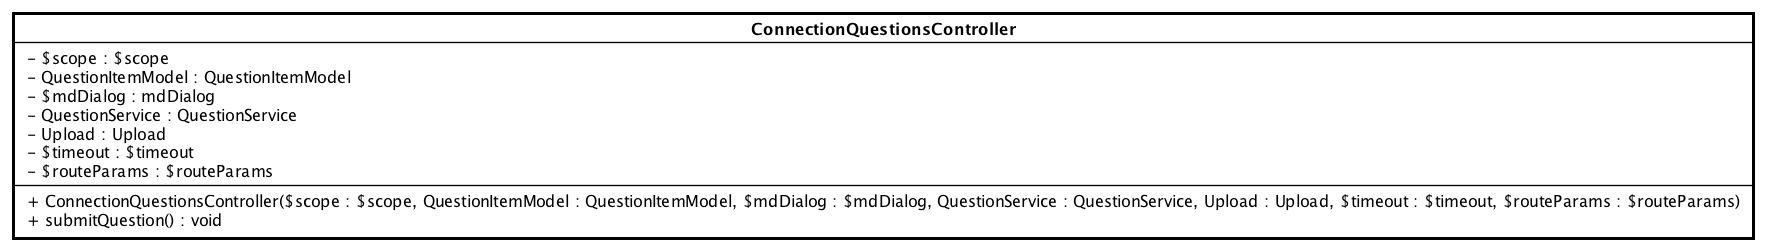
\includegraphics[scale=0.45]{UML/Classi/Front-End/QuizziPedia_Front-end_Controller_ConnectionQuestionsController.png}
	\caption{QuizziPedia::Front-End::Controllers::ConnectionQuestionsController}
\end{figure}
\begin{itemize}
	\item \textbf{Descrizione}: questa classe permette di gestire la creazione e la modifica di una domanda a collegamento;
	\item \textbf{Utilizzo}: fornisce le funzionalità per inserire una nuova domanda a collegamento nel database e per modificarne una esistente;
	\item \textbf{Relazione con altre classi:}
	\begin{itemize}
		\item \textit{IN} \texttt{ConnectionQuestionsView}: view contenente i campi per creare una domanda a collegamento;  
		\item \textit{OUT} \texttt{LangService}: questa classe permette di gestire la lingua nella quale si è scelto di utilizzare l'applicazione;
		\item \textit{OUT} \texttt{QuestionService}: questa classe permette di ottenere domande esistenti e salvare nuove domande;
		\item \textit{OUT} \texttt{ErrorController}: questa classe permette di gestire tutti i messaggi di errore da mostrare all'utente.
	\end{itemize}
	\item \textbf{Attributi:}
	\begin{itemize}
		\item 
	\end{itemize}
	\item \textbf{Metodi:}
	\begin{itemize}
		\item 
	\end{itemize}
\end{itemize}

\paragraph{QuizziPedia::Front-End::Controllers::ImagesSortingQuestionsController}
\begin{figure}
	\centering
	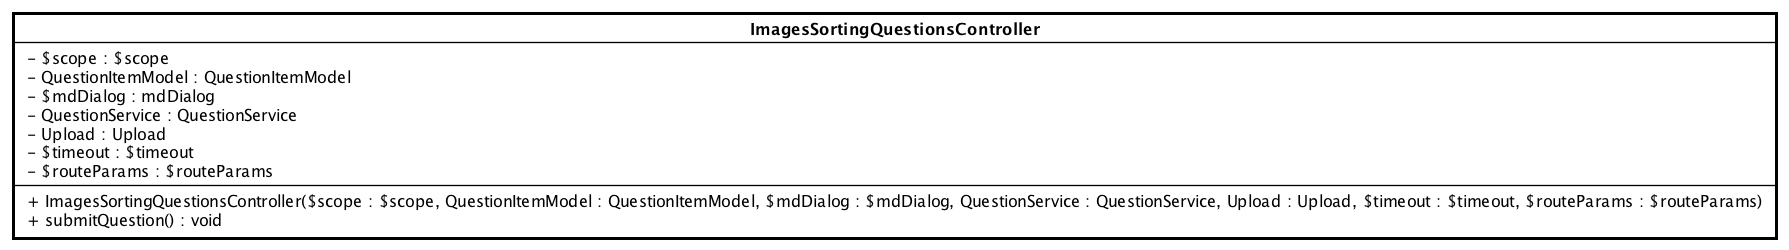
\includegraphics[scale=0.45]{UML/Classi/Front-End/QuizziPedia_Front-end_Controller_ImagesSortingQuestionsController.png}
	\caption{QuizziPedia::Front-End::Controllers::ImagesSortingQuestionsController}
\end{figure}
\begin{itemize}
	\item \textbf{Descrizione}: questa classe permette di gestire la creazione e la modifica di una domanda a ordinamento immagini;
	\item \textbf{Utilizzo}: fornisce le funzionalità per inserire una nuova domanda a ordinamento immagini nel database e per modificarne una esistente;
	\item \textbf{Relazione con altre classi:}
	\begin{itemize}
		\item \textit{IN} \texttt{ImagesSortingQuestionsView}: view contenente i campi per creare una domanda a ordinamento immagini; 
		\item \textit{OUT} \texttt{LangService}: questa classe permette di gestire la lingua nella quale si è scelto di utilizzare l'applicazione;
		\item \textit{OUT} \texttt{QuestionService}: questa classe permette di ottenere domande esistenti e salvare nuove domande;
		\item \textit{OUT} \texttt{ErrorController}: questa classe permette di gestire tutti i messaggi di errore da mostrare all'utente.
	\end{itemize}
	\item \textbf{Attributi:}
	\begin{itemize}
		\item 
	\end{itemize}
	\item \textbf{Metodi:}
	\begin{itemize}
		\item 
	\end{itemize}
\end{itemize}

\paragraph{QuizziPedia::Front-End::Controllers::StringsSortingQuestionsController}
\begin{figure}
	\centering
	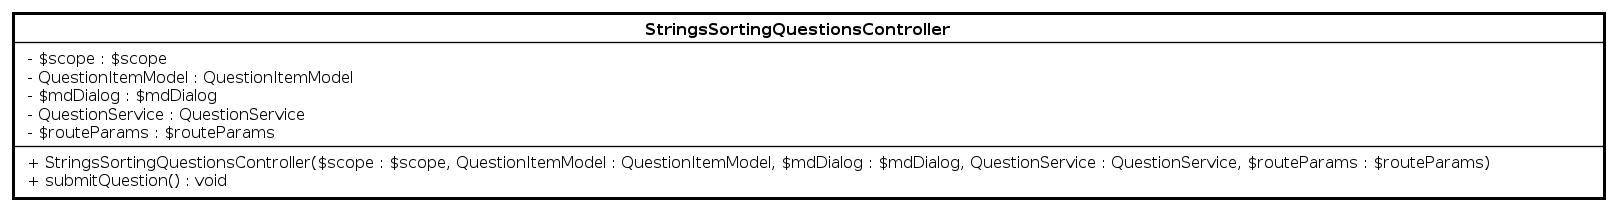
\includegraphics[scale=0.45]{UML/Classi/Front-End/QuizziPedia_Front-end_Controller_StringSortingQuestionsController.png}
	\caption{QuizziPedia::Front-End::Controllers::StringsSortingQuestionsController}
\end{figure}
\begin{itemize}
	\item \textbf{Descrizione}: questa classe permette di gestire la creazione e la modifica di una domanda a ordinamento di stringhe;
	\item \textbf{Utilizzo}: fornisce le funzionalità per inserire una nuova domanda a ordinamento di stringhe nel database e per modificarne una esistente;
	\item \textbf{Relazione con altre classi:}
	\begin{itemize}
		\item \textit{IN} \texttt{StringsSortingQuestionsView}: view contenente i campi per creare una domanda a ordinamento stringhe; 
		\item \textit{OUT} \texttt{LangService}: questa classe permette di gestire la lingua nella quale si è scelto di utilizzare l'applicazione;
		\item \textit{OUT} \texttt{QuestionService}: questa classe permette di ottenere domande esistenti e salvare nuove domande;
		\item \textit{OUT} \texttt{ErrorController}: questa classe permette di gestire tutti i messaggi di errore da mostrare all'utente.
	\end{itemize}
	\item \textbf{Attributi:}
	\begin{itemize}
		\item 
	\end{itemize}
	\item \textbf{Metodi:}
	\begin{itemize}
		\item 
	\end{itemize}
\end{itemize}

\paragraph{QuizziPedia::Front-End::Controllers::FillingQuestionsController}
\begin{figure}
	\centering
	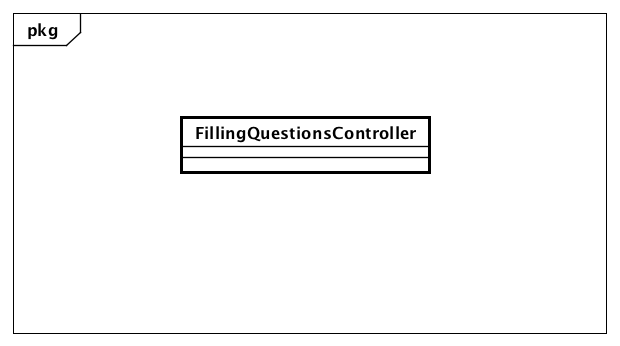
\includegraphics[scale=0.45]{UML/Classi/Front-End/QuizziPedia_Front-end_Controller_FillingQuestionsController.png}
	\caption{QuizziPedia::Front-End::Controllers::FillingQuestionsController}
\end{figure}
\begin{itemize}
	\item \textbf{Descrizione}: questa classe permette di gestire la creazione e la modifica di una domanda a riempimento di spazi;
	\item \textbf{Utilizzo}: fornisce le funzionalità per inserire una nuova domanda ariempimento di spazi nel database e per modificarne una esistente;
	\item \textbf{Relazione con altre classi:}
	\begin{itemize}
		\item \textit{IN} \texttt{FillingQuestionsView}: view contenente i campi per creare una domanda a riempimento testo; 
		\item \textit{OUT} \texttt{LangService}: questa classe permette di gestire la lingua nella quale si è scelto di utilizzare l'applicazione;
		\item \textit{OUT} \texttt{QuestionService}: questa classe permette di ottenere domande esistenti e salvare nuove domande;
		\item \textit{OUT} \texttt{ErrorController}: questa classe permette di gestire tutti i messaggi di errore da mostrare all'utente.
	\end{itemize}
	\item \textbf{Attributi:}
	\begin{itemize}
		\item 
	\end{itemize}
	\item \textbf{Metodi:}
	\begin{itemize}
		\item 
	\end{itemize}
\end{itemize}

\paragraph{QuizziPedia::Front-End::Controllers::ClickableAreaQuestionsController}
\begin{figure}
	\centering
	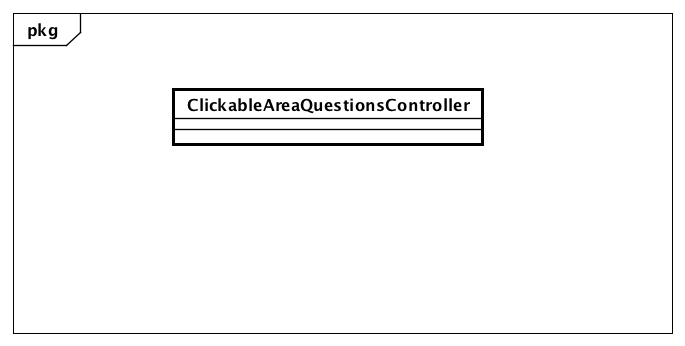
\includegraphics[scale=0.45]{UML/Classi/Front-End/QuizziPedia_Front-end_Controller_ClickableAreaQuestionsController.png}
	\caption{QuizziPedia::Front-End::Controllers::ClickableAreaQuestionsController}
\end{figure}
\begin{itemize}
	\item \textbf{Descrizione}: questa classe permette di gestire la creazione e la modifica di una domanda ad area cliccabile;
	\item \textbf{Utilizzo}: fornisce le funzionalità per inserire una nuova domanda ad area cliccabile nel database e per modificarne una esistente;
	\item \textbf{Relazione con altre classi:}
	\begin{itemize}
		\item \textit{IN} \texttt{ClickableAreaQuestionsView}: view contenente i campi per creare una domanda ad area cliccabile; 
		\item \textit{OUT} \texttt{LangService}: questa classe permette di gestire la lingua nella quale si è scelto di utilizzare l'applicazione;
		\item \textit{OUT} \texttt{QuestionService}: questa classe permette di ottenere domande esistenti e salvare nuove domande;
		\item \textit{OUT} \texttt{ErrorController}: questa classe permette di gestire tutti i messaggi di errore da mostrare all'utente.
	\end{itemize}
	\item \textbf{Attributi:}
	\begin{itemize}
		\item 
	\end{itemize}
	\item \textbf{Metodi:}
	\begin{itemize}
		\item 
	\end{itemize}
\end{itemize}

\paragraph{QuizziPedia::Front-End::Controllers::EditorQMLController}
\begin{figure}
	\centering
	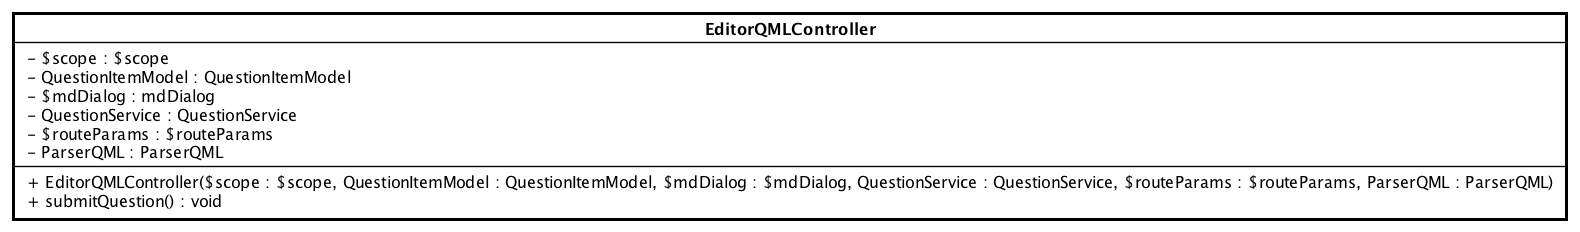
\includegraphics[scale=0.45]{UML/Classi/Front-End/QuizziPedia_Front-end_Controller_EditorQMLController.png}
	\caption{QuizziPedia::Front-End::Controllers::EditorQMLController}
\end{figure}
\begin{itemize}
	\item \textbf{Descrizione}: questa classe permette di gestire la creazione e la modifica di domande create tramite editor QML;
	\item \textbf{Utilizzo}: fornisce le funzionalità per creare e modificare una domanda tramite editor QML;
	\item \textbf{Relazione con altre classi:}
	\begin{itemize}
		\item \textit{IN} \texttt{EditorQMLView}: view contenente l'editor QML per la creazione di domande personalizzate; 
		\item \textit{OUT} \texttt{LangService}: questa classe permette di gestire la lingua nella quale si è scelto di utilizzare l'applicazione;
		\item \textit{OUT} \texttt{QuestionService}: questa classe permette di ottenere domande esistenti e salvare nuove domande;
		\item \textit{OUT} \texttt{ErrorController}: questa classe permette di gestire tutti i messaggi di errore da mostrare all'utente.
	\end{itemize}
	\item \textbf{Attributi:}
	\begin{itemize}
		\item 
	\end{itemize}
	\item \textbf{Metodi:}
	\begin{itemize}
		\item 
	\end{itemize}
\end{itemize}

\paragraph{QuizziPedia::Front-End::Controllers::QuestionsManagementController}
\begin{figure}
	\centering
	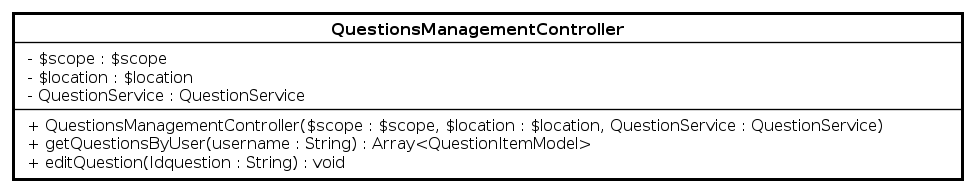
\includegraphics[scale=0.45]{UML/Classi/Front-End/QuizziPedia_Front-end_Controller_QuestionsManagementController.png}
	\caption{QuizziPedia::Front-End::Controllers::QuestionsManagementController}
\end{figure}
\begin{itemize}
	\item \textbf{Descrizione}: questa classe permette di gestire di ottenere le domande create dall'utente;
	\item \textbf{Utilizzo}: fornisce le funzionalità per richiedere al back-end le domande create dall'utente e mostrarle nella sua pagina personale; 
	\item \textbf{Relazione con altre classi:}
	\begin{itemize}
		\item \textit{IN} \texttt{QuestionsManagementView}: view contenente l'elenco delle domande create; 
		\item \textit{OUT} \texttt{LangService}: questa classe permette di gestire la lingua nella quale si è scelto di utilizzare l'applicazione;
		\item \textit{OUT} \texttt{QuestionService}: questa classe permette di ottenere domande esistenti e salvare nuove domande;
		\item \textit{OUT} \texttt{ErrorController}: questa classe permette di gestire tutti i messaggi di errore da mostrare all'utente.
	\end{itemize}
	\item \textbf{Attributi:}
	\begin{itemize}
		\item 
	\end{itemize}
	\item \textbf{Metodi:}
	\begin{itemize}
		\item 
	\end{itemize}
\end{itemize}

\paragraph{QuizziPedia::Front-End::Controllers::TrainingController}
\begin{figure}
	\centering
	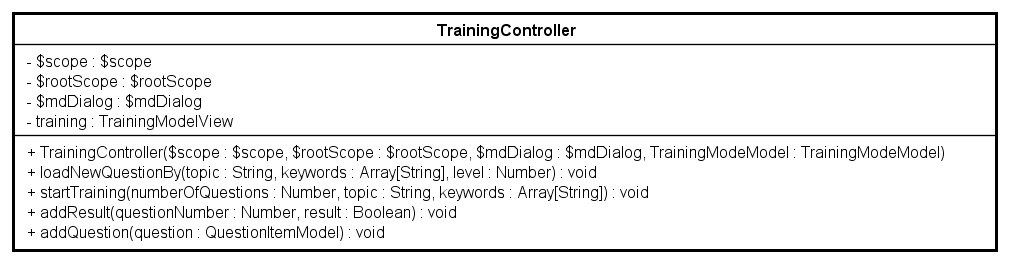
\includegraphics[scale=0.45]{UML/Classi/Front-End/QuizziPedia_Front-end_Controller_TrainingController.png}
	\caption{QuizziPedia::Front-End::Controllers::TrainingController}
\end{figure}
\begin{itemize}
	\item \textbf{Descrizione}: questa classe permette di gestire la modalità allenamento sottoponendo all'utente le giuste domande adatte al suo livello;
	\item \textbf{Utilizzo}: fornisce le funzionalità per recuperare le domande che siano in accordo con il livello dell'utente;
	\item \textbf{Relazione con altre classi:}
	\begin{itemize}
		\item \textit{IN} \texttt{TrainingView}: view principale della modalità allenamento;
		\item \textit{IN} \texttt{TrainingSetUpTemplate}: rappresenta il componente grafico che permette all'utente di selezionare l'argomento e le parole chiave per iniziare un allenamento con queste caratteristiche. Viene gestito dinamicamente all'interno della view TrainingView attraverso il controller TrainingController;
		\item \textit{OUT} \texttt{LangService}: questa classe permette di gestire la lingua nella quale si è scelto di utilizzare l'applicazione;
		\item \textit{OUT} \texttt{ErrorController}: questa classe permette di gestire tutti i messaggi di errore da mostrare all'utente.
	\end{itemize}
	\item \textbf{Attributi:}
	\begin{itemize}
		\item 
	\end{itemize}
	\item \textbf{Metodi:}
	\begin{itemize}
		\item 
	\end{itemize}
\end{itemize}

\paragraph{QuizziPedia::Front-End::Controllers::FillingQuestionnaireController}
\begin{figure}
	\centering
	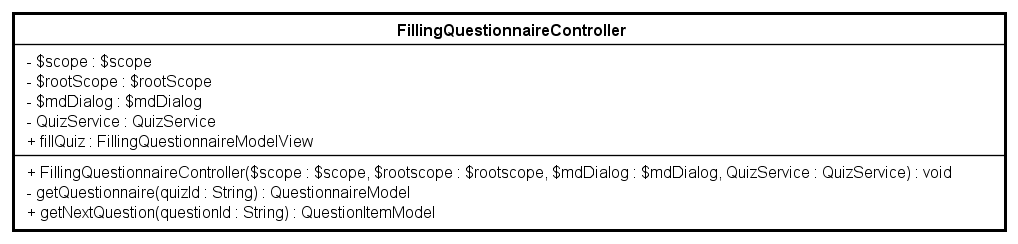
\includegraphics[scale=0.45]{UML/Classi/Front-End/QuizziPedia_Front-end_Controller_FillingQuestionnaireController.png}
	\caption{QuizziPedia::Front-End::Controllers::FillingQuestionnaireController}
\end{figure}
\begin{itemize}
	\item \textbf{Descrizione}: questa classe permette di gestire la compilazione del questionario;
	\item \textbf{Utilizzo}: fornisce le funzionalità per compilare un questionario e per gestire il cambio di domanda;
	\item \textbf{Relazione con altre classi:}
	\begin{itemize}
		\item \textit{IN} \texttt{FillingQuestionnaireView}: view principale per la compilazione del questionario;  
		\item \textit{IN} \texttt{InfoQuestionnaireTemplate}: rappresenta il componente grafico che permette all'utente di visualizzare le informazioni principali del questionario che si sta per svolgere. Viene gestito dinamicamente all'interno della view TrainingView attraverso il controller TrainingController;
		\item \textit{OUT} \texttt{LangService}: questa classe permette di gestire la lingua nella quale si è scelto di utilizzare l'applicazione;
		\item \textit{OUT} \texttt{QuizService}: questa classe permette di ottenere i dati di un quiz tramite delle parole chiave inserite dall'utente nella barra di ricerca;
		\item \textit{OUT} \texttt{ErrorController}: questa classe permette di gestire tutti i messaggi di errore da mostrare all'utente.
	\end{itemize}
	\item \textbf{Attributi:}
	\begin{itemize}
		\item 
	\end{itemize}
	\item \textbf{Metodi:}
	\begin{itemize}
		\item 
	\end{itemize}
\end{itemize}

\paragraph{QuizziPedia::Front-End::Controllers::CreateQuestionnaireController}
\begin{figure}
	\centering
	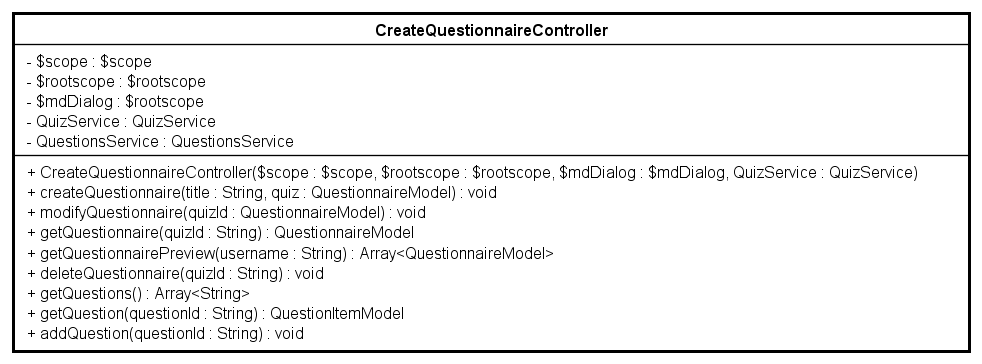
\includegraphics[scale=0.45]{UML/Classi/Front-End/QuizziPedia_Front-end_Controller_CreateQuestionnaireController.png}
	\caption{QuizziPedia::Front-End::Controllers::CreateQuestionnaireController}
\end{figure}
\begin{itemize}
	\item \textbf{Descrizione}: questa classe permette di gestire la creazione di un questionario;
	\item \textbf{Utilizzo}: fornisce tutte le funzionalità per la creazione di un nuovo questionario e per la modifica di uno esistente;
	\item \textbf{Relazione con altre classi:}
	\begin{itemize}
		\item \textit{IN} \texttt{CreateQuestionnaireView}: view per la creazione del questionario; 
		\item \textit{OUT} \texttt{QuizService}: questa classe permette di ottenere i dati di un quiz tramite delle parole chiave inserite dall'utente nella barra di ricerca;
		\item \textit{OUT} \texttt{LangService}: questa classe permette di gestire la lingua nella quale si è scelto di utilizzare l'applicazione;
		\item \textit{OUT} \texttt{ErrorController}: questa classe permette di gestire tutti i messaggi di errore da mostrare all'utente.
	\end{itemize}
	\item \textbf{Attributi:}
	\begin{itemize}
		\item 
	\end{itemize}
	\item \textbf{Metodi:}
	\begin{itemize}
		\item 
	\end{itemize}
\end{itemize}

\paragraph{QuizziPedia::Front-End::Controllers::RegistrationManagementController}
\begin{figure}
	\centering
	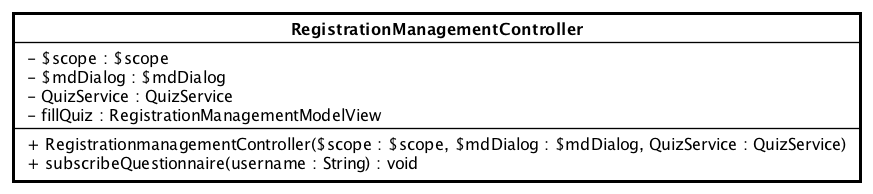
\includegraphics[scale=0.45]{UML/Classi/Front-End/QuizziPedia_Front-end_Controller_RegistrationManagementController.png}
	\caption{QuizziPedia::Front-End::Controllers::RegistrationManagementController}
\end{figure}
\begin{itemize}
	\item \textbf{Descrizione}: questa classe permette di gestire le iscrizione degli utenti ai questionari;
	\item \textbf{Utilizzo}: fornisce le funzionalità di iscrizione ad un questionario;
	\item \textbf{Relazione con altre classi:}
	\begin{itemize}
		\item \textit{IN} \texttt{RegistratioManagementView}: view per la gestione degli utenti iscritti a un proprio questionario; 
		\item \textit{OUT} \texttt{QuizService}: questa classe permette di ottenere i dati di un quiz tramite delle parole chiave inserite dall'utente nella barra di ricerca;
		\item \textit{OUT} \texttt{LangService}: questa classe permette di gestire la lingua nella quale si è scelto di utilizzare l'applicazione;
		\item \textit{OUT} \texttt{ErrorController}: questa classe permette di gestire tutti i messaggi di errore da mostrare all'utente.
	\end{itemize}
	\item \textbf{Attributi:}
	\begin{itemize}
		\item 
	\end{itemize}
	\item \textbf{Metodi:}
	\begin{itemize}
		\item 
	\end{itemize}
\end{itemize}

\paragraph{QuizziPedia::Front-End::Controllers::ResultsController}
\begin{figure}
	\centering
	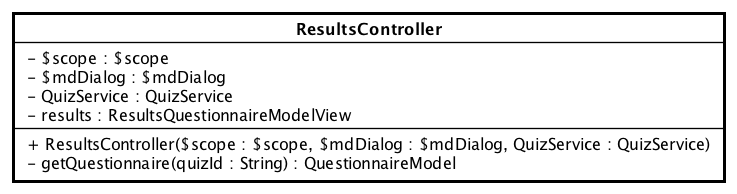
\includegraphics[scale=0.45]{UML/Classi/Front-End/QuizziPedia_Front-end_Controller_ResultsController.png}
	\caption{QuizziPedia::Front-End::Controllers::ResultsController}
\end{figure}
\begin{itemize}
	\item \textbf{Descrizione}: questa classe permette di gestire i risultati della ricerca effettuata dall'utente;
	\item \textbf{Utilizzo}: fornisce le funzionalità per recuperare i dati dal back-end e mostrarli all'utente nella view;
	\item \textbf{Relazione con altre classi:}
	\begin{itemize}
		\item \textit{IN} \texttt{ResultsView}: view contenente i risultati della ricerca effettuata, sia gli utenti che i questionari; 
		\item \textit{OUT} \texttt{QuizService}: questa classe permette di ottenere i dati di un quiz tramite delle parole chiave inserite dall'utente nella barra di ricerca;
		\item \textit{OUT} \texttt{LangService}: questa classe permette di gestire la lingua nella quale si è scelto di utilizzare l'applicazione;
		\item \textit{OUT} \texttt{ErrorController}: questa classe permette di gestire tutti i messaggi di errore da mostrare all'utente.
	\end{itemize}
	\item \textbf{Attributi:}
	\begin{itemize}
		\item 
	\end{itemize}
	\item \textbf{Metodi:}
	\begin{itemize}
		\item 
	\end{itemize}
\end{itemize}

\paragraph{QuizziPedia::Front-End::Controllers::QuestionnaireManagementController}
\begin{figure}
	\centering
	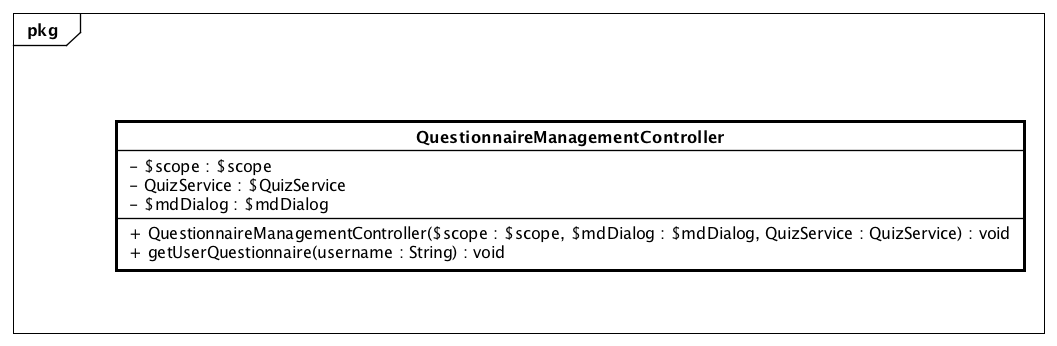
\includegraphics[scale=0.45]{UML/Classi/Front-End/QuizziPedia_Front-end_Controller_QuestionnaireManagementController.png}
	\caption{QuizziPedia::Front-End::Controllers::QuestionnaireManagementController}
\end{figure}
\begin{itemize}
	\item \textbf{Descrizione}: questa classe permette di gestire tutti i questionari creati da un utente; 
	\item \textbf{Utilizzo}: fornisce le funzionalità per recuperare dal back-end tutti i questionari creati da un utente;
	\item \textbf{Relazione con altre classi:}
	\begin{itemize}
		\item \textit{IN} \texttt{QuestionnaireManagementeView}: view principale per la gestione dei questionari;
		\item \textit{OUT} \texttt{QuizService}: questa classe permette di ottenere i dati di un quiz tramite delle parole chiave inserite dall'utente nella barra di ricerca;
		\item \textit{OUT} \texttt{LangService}: questa classe permette di gestire la lingua nella quale si è scelto di utilizzare l'applicazione;
		\item \textit{OUT} \texttt{ErrorController}: questa classe permette di gestire tutti i messaggi di errore da mostrare all'utente.
	\end{itemize}
	\item \textbf{Attributi:}
	\begin{itemize}
		\item 
	\end{itemize}
	\item \textbf{Metodi:}
	\begin{itemize}
		\item 
	\end{itemize}
\end{itemize}

\paragraph{QuizziPedia::Front-End::Controllers::MenuBarController}
\begin{figure}
	\centering
	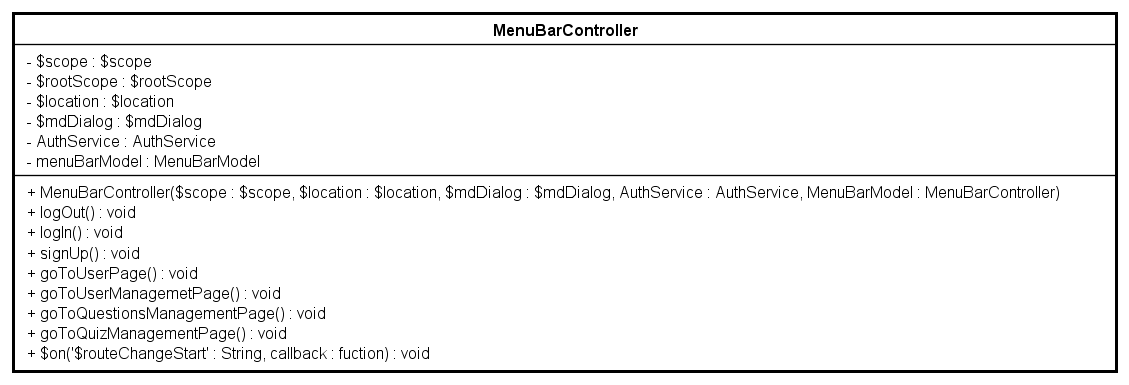
\includegraphics[scale=0.45]{UML/Classi/Front-End/QuizziPedia_Front-end_Controller_MenuBarController.png}
	\caption{QuizziPedia::Front-End::Controllers::MenuBarController}
\end{figure}
\begin{itemize}
	\item \textbf{Descrizione}: questa classe permette di gestire il menù fisso per ogni pagina;
	\item \textbf{Utilizzo}: fornisce le funzionalità per aggiornare, a seconda della pagina, il contenuto del menù;
	\item \textbf{Relazione con altre classi:}
	\begin{itemize}
		\item \textit{IN} \texttt{MenuBarDirective}: rappresenta il menù, presente in ogni pagina dell'applicazione, generato in base agli oggetti passati nello \$scope isolato. Fornisce un pulsante per ogni oggetto ricevuto come parametro, ogni pulsante viene rappresentato con un’icona e con un testo. Al click di un pulsante viene invocata la funzione ad esso associata;  
		\item \textit{OUT} \texttt{LangService}: questa classe permette di gestire la lingua nella quale si è scelto di utilizzare l'applicazione;
		\item \textit{OUT} \texttt{ErrorController}: questa classe permette di gestire tutti i messaggi di errore da mostrare all'utente.
	\end{itemize}
	\item \textbf{Attributi:}
	\begin{itemize}
		\item 
	\end{itemize}
	\item \textbf{Metodi:}
	\begin{itemize}
		\item 
	\end{itemize}
\end{itemize}

\paragraph{QuizziPedia::Front-End::Controllers::FooterController}
\begin{figure}
	\centering
	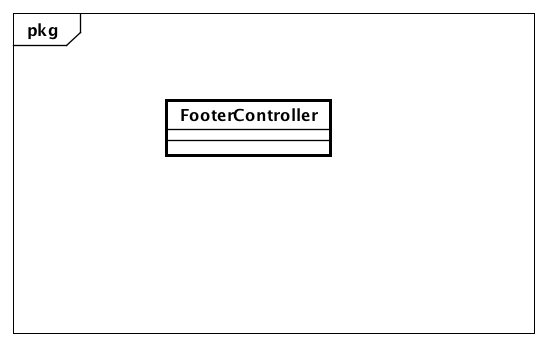
\includegraphics[scale=0.45]{UML/Classi/Front-End/QuizziPedia_Front-end_Controller_FooterController.png}
	\caption{QuizziPedia::Front-End::Controllers::FooterController}
\end{figure}
\begin{itemize}
	\item \textbf{Descrizione}: questa classe permette di gestire il footer dell'applicazione;
	\item \textbf{Utilizzo}: fornisce le funzionalità per recuperare le informazioni da mostrare nel footer;
	\item \textbf{Relazione con altre classi:}
	\begin{itemize}
		\item \textit{IN} \texttt{FooterDirective}: directive che mostra il footer dell'applicazione che sarà presente in ogni pagina;  
		\item \textit{OUT} \texttt{LangService}: questa classe permette di gestire la lingua nella quale si è scelto di utilizzare l'applicazione;
		\item \textit{OUT} \texttt{ErrorController}: questa classe permette di gestire tutti i messaggi di errore da mostrare all'utente.
	\end{itemize}
	\item \textbf{Attributi:}
	\begin{itemize}
		\item 
	\end{itemize}
	\item \textbf{Metodi:}
	\begin{itemize}
		\item 
	\end{itemize}
\end{itemize}

\paragraph{QuizziPedia::Front-End::Controllers::ErrorController}
\begin{figure}
	\centering
	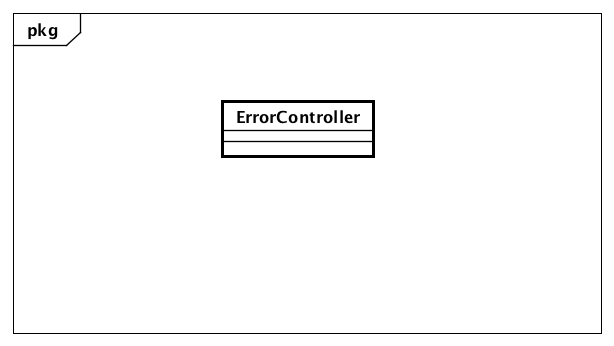
\includegraphics[scale=0.45]{UML/Classi/Front-End/QuizziPedia_Front-end_Controller_ErrorController.png}
	\caption{QuizziPedia::Front-End::Controllers::ErrorController}
\end{figure}
\begin{itemize}
	\item \textbf{Descrizione}: questa classe permette di gestire tutti i messaggi di errore da mostrare all'utente;
	\item \textbf{Utilizzo}: fornisce le funzionalità che permettono di recuperare il giusto messaggio di errore ad ogni situazione anomala;
	\item \textbf{Relazione con altre classi:}
	\begin{itemize}
		\item \textit{IN} \texttt{ErrorDirective}: directive che mostra l'eventuale errore dopo un'azione;
		\item \textit{IN} \texttt{LoginController}: questa classe permette di gestire l'autenticazione dell'utente al sistema; 
		\item \textit{IN} \texttt{PasswordForgotController}: questa classe permette di gestire il ripristino della password dimenticata;
		\item \textit{IN} \texttt{SignUpController}: questa classe permette di gestire la registrazione di un utente al sistema;
		\item \textit{IN} \texttt{SearchController}: questa classe permette di gestire la ricerca di questionari e utenti all'interno dell'applicazione;
		\item \textit{OUT} \texttt{LangService}: questa classe permette di gestire la lingua nella quale si è scelto di utilizzare l'applicazione;
		\item \textit{OUT} \texttt{ErrorService}: questa classe permette di gestire il recupero e la gestione dei messaggi di errore;
		\item \textit{OUT} \texttt{ErrorInfoModel}: rappresenta le informazioni di un errore che si è verificato eseguendo una determinata operazione.
	\end{itemize}
	\item \textbf{Attributi:}
	\begin{itemize}
		\item 
	\end{itemize}
	\item \textbf{Metodi:}
	\begin{itemize}
		\item 
	\end{itemize}
\end{itemize}

\paragraph{QuizziPedia::Front-End::Controllers::QuestionnaireDetailsController}
\begin{figure}
	\centering
	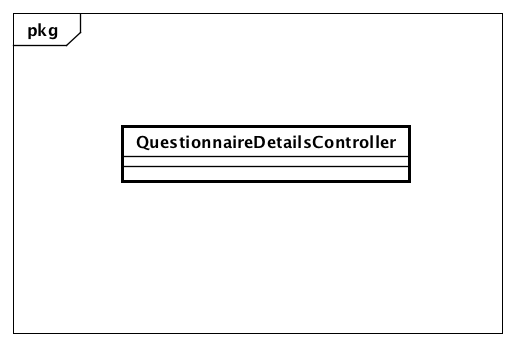
\includegraphics[scale=0.45]{UML/Classi/Front-End/QuizziPedia_Front-end_Controller_QuestionnaireDetailsController.png}
	\caption{QuizziPedia::Front-End::Controllers::QuestionnaireDetailsController}
\end{figure}
\begin{itemize}
	\item \textbf{Descrizione}: questa classe permette di gestire i dettagli di un questionario; 
	\item \textbf{Utilizzo}: fornisce le funzionalità per recuperare dal back-end i dettagli di un questionario creato da un utente al fine di poterli visualizzare nel suo profilo;
	\item \textbf{Relazione con altre classi:}
	\begin{itemize}
		\item \textit{IN} \texttt{QuestionnaireDetailsDirective}: rappresenta il componente grafico che permette all'utente di visualizzare la lista di questionari che può compilare;
		\item \textit{OUT} \texttt{QuizService}: questa classe permette di ottenere i dati di un quiz tramite delle parole chiave inserite dall'utente nella barra di ricerca;
		\item \textit{OUT} \texttt{ErrorController}: questa classe permette di gestire tutti i messaggi di errore da mostrare all'utente.
	\end{itemize}
	\item \textbf{Attributi:}
	\begin{itemize}
		\item 
	\end{itemize}
	\item \textbf{Metodi:}
	\begin{itemize}
		\item 
	\end{itemize}
\end{itemize}

\paragraph{QuizziPedia::Front-End::Controllers::UserDetailController}
\begin{figure}
	\centering
	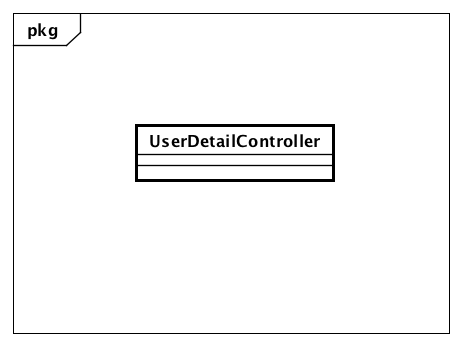
\includegraphics[scale=0.45]{UML/Classi/Front-End/QuizziPedia_Front-end_Controller_UserDetailController.png}
	\caption{QuizziPedia::Front-End::Controllers::UserDetailController}
\end{figure}
\begin{itemize}
	\item \textbf{Descrizione}: questa classe permette di gestire i dati di un utente;
	\item \textbf{Utilizzo}: fornisce le funzionalità per recuperare i dati di un utente, visualizzabili sia come dati personali dell'utente che ha effettuato l'accesso sia come risultato di una ricerca per utenti;
	\item \textbf{Relazione con altre classi:}
	\begin{itemize}
		\item \textit{IN} \texttt{UserDetailsDirective}: directive che permette di visualizzare i dati personali di un utente;
		\item \textit{OUT} \texttt{UserDetailsService}: questa classe permette di ottenere domande esistenti e salvare nuove domande;
		\item \textit{OUT} \texttt{ErrorController}: questa classe permette di gestire tutti i messaggi di errore da mostrare all'utente.

	\end{itemize}
	\item \textbf{Attributi:}
	\begin{itemize}
		\item 
	\end{itemize}
	\item \textbf{Metodi:}
	\begin{itemize}
		\item 
	\end{itemize}
\end{itemize}

\paragraph{QuizziPedia::Front-End::Controllers::QuestionsController}
\begin{figure}
	\centering
	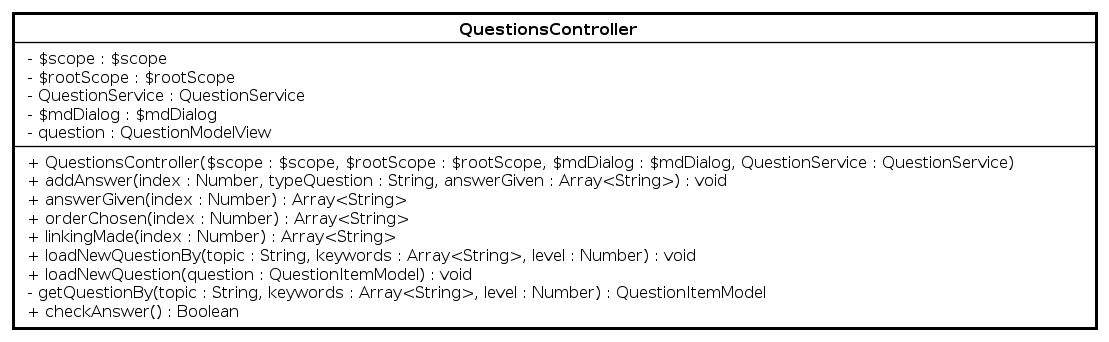
\includegraphics[scale=0.45]{UML/Classi/Front-End/QuizziPedia_Front-end_Controller_QuestionsController.png}
	\caption{QuizziPedia::Front-End::Controllers::QuestionsController}
\end{figure}
\begin{itemize}
	\item \textbf{Descrizione}: questa classe permette di gestire il recupero delle domande per poterle stampare nella modalità allenamento;
	\item \textbf{Utilizzo}: fornisce le funzionalità per il recupero delle domande esistenti nel database al fine di mostrarle durante la modalità allenamento nell'apposito template;
	\item \textbf{Relazione con altre classi:}
	\begin{itemize}
		\item \textit{IN} \texttt{HeaderTextQuestionTemplate}: rappresenta il componente grafico che presenta all'utente il testo della domanda, l'argomento e le parole chiave. Viene gestito dinamicamente all'interno della view TrainingView attraverso il controller TrainingController; 
		\item \textit{IN} \texttt{TrueFalseAnswerTemplate}: rappresenta il componente grafico che permette all'utente di visualizzare la domanda vero e falso. Viene gestito dinamicamente all'interno della view TrainingView attraverso il controller TrainingController; 
		\item \textit{IN} \texttt{MultipleChoiceAnswerTemplate}: rappresenta il componente grafico che permette all'utente di visualizzare la domanda a risposta multipla. Viene gestito dinamicamente all'interno della view TrainingView attraverso il controller TrainingController; 
		\item \textit{IN} \texttt{LinkingAnswerTemplate}: rappresenta il componente grafico che permette all'utente di visualizzare la domanda di collegamento. Viene gestito dinamicamente all'interno della view TrainingView attraverso il controller TrainingController; 
		\item \textit{IN} \texttt{SortImagesAnswerTemplate}: rappresenta il componente grafico che permette all'utente di visualizzare la domanda ad ordinamento di immagini. Viene gestito dinamicamente all'interno della view TrainingView attraverso il controller TrainingController; 
		\item \textit{IN} \texttt{SortTextAnswerTemplate}: rappresenta il componente grafico che permette all'utente di visualizzare la domanda ad ordinamento di stringhe. Viene gestito dinamicamente all'interno della view TrainingView attraverso il controller TrainingController; 
		\item \textit{IN} \texttt{EmptySpaceAnswerTemnplate}: rappresenta il componente grafico che permette all'utente di visualizzare l'esercizio a riempimento di spazi vuoti. Viene gestito dinamicamente all'interno della view TrainingView attraverso il controller TrainingController; 
		\item \textit{IN} \texttt{ClickableAnswerTemplate}: rappresenta il componente grafico che permette all'utente di visualizzare la domanda ad area cliccabile nell'immagine. Viene gestito dinamicamente all'interno della view TrainingView attraverso il controller TrainingController;  
		\item \textit{OUT} \texttt{QuestionServices}: questa classe permette di ottenere domande esistenti e salvare nuove domande;
		\item \textit{OUT} \texttt{ErrorController}: questa classe permette di gestire tutti i messaggi di errore da mostrare all'utente.
	\end{itemize}
	\item \textbf{Attributi:}
	\begin{itemize}
		\item 
	\end{itemize}
	\item \textbf{Metodi:}
	\begin{itemize}
		\item 
	\end{itemize}
\end{itemize}

\paragraph{QuizziPedia::Front-End::Controllers::TopicKeywordsController}
\begin{figure}
	\centering
	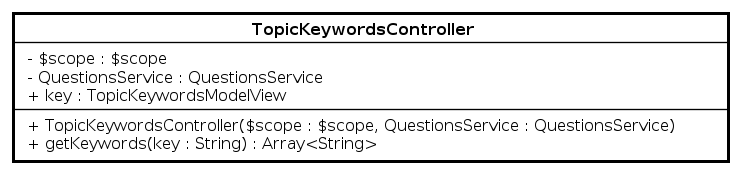
\includegraphics[scale=0.45]{UML/Classi/Front-End/QuizziPedia_Front-end_Controller_TopicKeywordsController.png}
	\caption{QuizziPedia::Front-End::Controllers::TopicKeywordsController}
\end{figure}
\begin{itemize}
	\item \textbf{Descrizione}: questa classe permette di gestire il recupero delle parole chiave di un questionario;
	\item \textbf{Utilizzo}: fornisce le funzionalità per il recupero delle parole chiave durante la creazione di un questionario;
	\item \textbf{Relazione con altre classi:}
	\begin{itemize}
		\item \textit{IN} \texttt{TopicKeywordsDirective}: directive che permette di gestire l'inserimento di keywords al momento della creazione della domanda; 
		\item \textit{IN} \texttt{QuestionsService}: questa classe permette di ottenere domande esistenti e salvare nuove domande; 
		\item \textit{OUT} \texttt{ErrorController}: questa classe permette di gestire tutti i messaggi di errore da mostrare all'utente.
	\end{itemize}
	\item \textbf{Attributi:}
	\begin{itemize}
		\item 
	\end{itemize}
	\item \textbf{Metodi:}
	\begin{itemize}
		\item 
	\end{itemize}
\end{itemize}

\paragraph{QuizziPedia::Front-End::Controllers::QuestionnaireQuestionsManagementController}
\begin{figure}
	\centering
	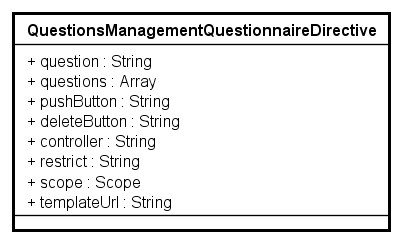
\includegraphics[scale=0.45]{UML/Classi/Front-End/QuizziPedia_Front-end_Controller_QuestionnaireQuestionsManagementController.png}
	\caption{QuizziPedia::Front-End::Controllers::QuestionnaireQuestionsManagementController}
\end{figure}
\begin{itemize}
	\item \textbf{Descrizione}: questa classe permette di gestire il recupero delle domande per il questionario;
	\item \textbf{Utilizzo}: fornisce le funzionalità per il recupero delle domande dal back-end e le rende disponibili per poter popolare le view;
	\item \textbf{Relazione con altre classi:}
	\begin{itemize}
		\item \textit{IN} \texttt{QuestionnaireQuestionsManagementDirective}: rappresenta il componente grafico che permette all'utente di:
		\begin{itemize}
			\item Effettuare delle ricerche sul database di domande;
			\item Selezionare le domande da inserire nel questionario;
			\item Mostrare le domande già inserite e permettere all'utente di eliminarle da tale lista.
		\end{itemize}
		Questo componente si presta sia per la creazione che per la modifica di un questionario;
		\item \textit{IN} \texttt{QuestionsService}: questa classe permette di ottenere domande esistenti e salvare nuove domande;
		\item \textit{OUT} \texttt{ErrorController}: questa classe permette di gestire tutti i messaggi di errore da mostrare all'utente.
	\end{itemize}
	\item \textbf{Attributi:}
	\begin{itemize}
		\item 
	\end{itemize}
	\item \textbf{Metodi:}
	\begin{itemize}
		\item 
	\end{itemize}
\end{itemize}

\paragraph{QuizziPedia::Front-End::Controllers::InputToListController}
\begin{figure}
	\centering
	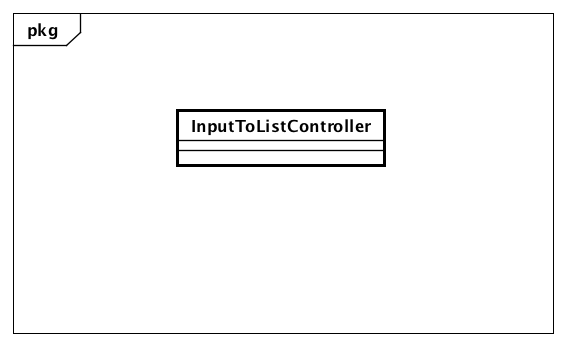
\includegraphics[scale=0.45]{UML/Classi/Front-End/QuizziPedia_Front-end_Controller_InputToListController.png}
	\caption{QuizziPedia::Front-End::Controllers::InputToListController}
\end{figure}
\begin{itemize}
	\item \textbf{Descrizione}: questa classe permette di gestire l'inserimento di una lista di risposte durante la creazione di una domanda;
	\item \textbf{Utilizzo}: fornisce le funzionalità per confermare porzioni di domanda durante la creazione;
	\item \textbf{Relazione con altre classi:}
	\begin{itemize}
		\item \textit{IN} \texttt{ConnectionQuestionsView}: view contenente i campi per creare una domanda a collegamento;
		\item \textit{IN} \texttt{StringsSortingQuestionsView}: view contenente i campi per creare una domanda a ordinamento stringhe; 
		\item \textit{IN} \texttt{ImagesSortingQuestionsView}: view contenente i campi per creare una domanda a ordinamento immmagini;
		\item \textit{OUT} \texttt{ErrorController}: questa classe permette di gestire tutti i messaggi di errore da mostrare all'utente. 
	\end{itemize}
	\item \textbf{Attributi:}
	\begin{itemize}
		\item 
	\end{itemize}
	\item \textbf{Metodi:}
	\begin{itemize}
		\item 
	\end{itemize}
\end{itemize}

\paragraph{QuizziPedia::Front-End::Controllers::NewQuestionsButtonController}
\begin{figure}
	\centering
	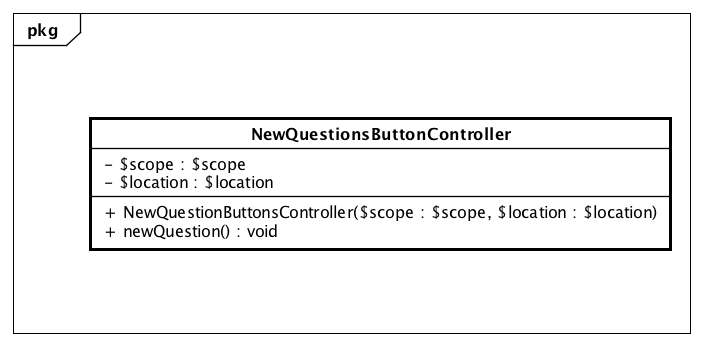
\includegraphics[scale=0.45]{UML/Classi/Front-End/QuizziPedia_Front-end_Controller_NewQuestionsButtonController.png}
	\caption{QuizziPedia::Front-End::Controllers::NewQuestionButtonController}
\end{figure}
\begin{itemize}
	\item \textbf{Descrizione}: questa classe permette di effettuare il redirect alla pagina di creazione nuova domanda;
	\item \textbf{Utilizzo}: effettua il redirect alla pagina di creazione nuova domanda quando l'utente seleziona l'apposito link;
	\item \textbf{Relazione con altre classi:}
	\begin{itemize}
		\item \textit{IN} \texttt{NewQuestionButtonsDirective}: rappresenta il componente grafico che permette all'utente di posizionarsi nella view di creazione di una nuova domanda; 
		\item \textit{OUT} \texttt{ErrorController}: questa classe permette di gestire tutti i messaggi di errore da mostrare all'utente.
	\end{itemize}
	\item \textbf{Attributi:}
	\begin{itemize}
		\item 
	\end{itemize}
	\item \textbf{Metodi:}
	\begin{itemize}
		\item 
	\end{itemize}
\end{itemize}

\paragraph{QuizziPedia::Front-End::Controllers::StatisticsController}
\begin{figure}
	\centering
	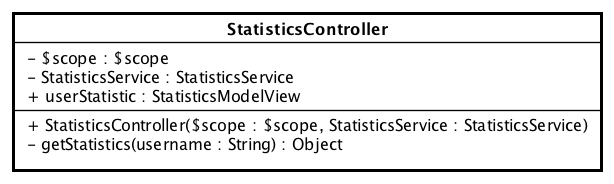
\includegraphics[scale=0.45]{UML/Classi/Front-End/QuizziPedia_Front-end_Controller_StatisticsController.png}
	\caption{QuizziPedia::Front-End::Controllers::StatisticsController}
\end{figure}
\begin{itemize}
	\item \textbf{Descrizione}: questa classe permette di le statistiche di un utente;
	\item \textbf{Utilizzo}: fornisce le funzionalità per ottenere le statistiche di un utente per poterle mostrare nella view;
	\item \textbf{Relazione con altre classi:}
	\begin{itemize}
		\item \textit{IN} \texttt{StatisticsDirective}: directive che permette di visualizzare le statistiche di un utente; 
		\item \textit{OUT} \texttt{StatisticsService}: questa classe permette di ottenere le statistiche dell'utente;
		\item \textit{OUT} \texttt{ErrorController}: questa classe permette di gestire tutti i messaggi di errore da mostrare all'utente.
	\end{itemize}
	\item \textbf{Attributi:}
	\begin{itemize}
		\item 
	\end{itemize}
	\item \textbf{Metodi:}
	\begin{itemize}
		\item 
	\end{itemize}
\end{itemize}

\paragraph{QuizziPedia::Front-End::Controllers::QuizEventController}
\begin{figure}
	\centering
	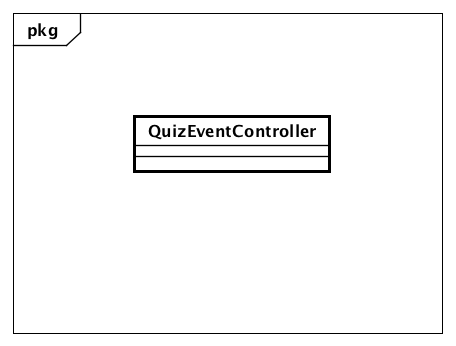
\includegraphics[scale=0.45]{UML/Classi/Front-End/QuizziPedia_Front-end_Controller_QuizEventController.png}
	\caption{QuizziPedia::Front-End::Controllers::QuizEventController}
\end{figure}
\begin{itemize}
	\item \textbf{Descrizione}: questa classe permette di reagire ai comandi dell'utente durante la gestione dei suoi questionari;
	\item \textbf{Utilizzo}: fornisce le funzionalità per reagire ai comandi dell'utente, effettua redirect alle pagine richieste, come la visualizzazione delle statistiche di un questionario e iniziare un questionario in modalità esame.
	\item \textbf{Relazione con altre classi:}
	\begin{itemize}
		\item \textit{IN} \texttt{CreationAndModifyDirective}:  
		\item \textit{OUT} \texttt{ExamModalityDirective}:
		\item \textit{OUT} \texttt{ErrorController}: questa classe permette di gestire tutti i messaggi di errore da mostrare all'utente.
	\end{itemize}
	\item \textbf{Attributi:}
	\begin{itemize}
		\item 
	\end{itemize}
	\item \textbf{Metodi:}
	\begin{itemize}
		\item 
	\end{itemize}
\end{itemize}